\documentclass[11pt]{article}
% amsmath package, useful for mathematical formulas
\usepackage{amsmath}
%\usepackage{natbib}
% amssymb package, useful for mathematical symbols
\usepackage{amssymb}
\usepackage{booktabs}
\usepackage{xspace}
% graphicx package, useful for including eps and pdf graphics
% include graphics with the command \includegraphics
\usepackage{graphicx}


% cite package, to clean up citations in the main text. Do not remove.
\usepackage{cite}
\usepackage{caption}
\usepackage{subcaption}

\usepackage{color} 

% Use doublespacing - comment out for single spacing
%\usepackage{setspace} 
%\doublespacing


% Text layout
\topmargin 0.0cm
\oddsidemargin 0.5cm
\evensidemargin 0.5cm
\textwidth 16cm 
\textheight 21cm

% Bold the 'Figure #' in the caption and separate it with a period
% Captions will be left justified
\usepackage[labelfont=bf,labelsep=period,justification=raggedright]{caption}

% Use the PLoS provided bibtex style
\bibliographystyle{/Users/stephens/Dropbox/Documents/stylefiles/plos2009}

% Remove brackets from numbering in List of References
\makeatletter
\renewcommand{\@biblabel}[1]{\quad#1.}
\makeatother


% Leave date blank
\date{}

\pagestyle{myheadings}
%% ** EDIT HERE **
\usepackage{enumerate}
\usepackage{multirow} 
\usepackage{url}
\usepackage{xr} %for cross-referencing
%% ** EDIT HERE **
%% PLEASE INCLUDE ALL MACROS BELOW
\newtheorem{algorithm}{Algorithm}
\newtheorem{proposition}{Proposition}
\newtheorem{restateproposition}{Proposition}
\newtheorem{lemma}{Lemma}
\newtheorem{corollary}{Corollary}
\newtheorem{result}{Result}
\newtheorem{note}{Note}
\newtheorem{definition}{Definition}

\begin{document}

\section{Ancient Structure Report}

\subsection{Introduction}

We want  to develop an analogous model to STRUCTURE for ancient DNA data that borrowed information from ancient DNA data to define the clusters in pooled modern + ancient SNP data. We first became interested in this from reading Haak et al 2015 in which they claimed that modern Europeans can be written as a mixture of 3 ancestral source populations and produced the following figure (Fig 1).

\begin{figure}[ht]
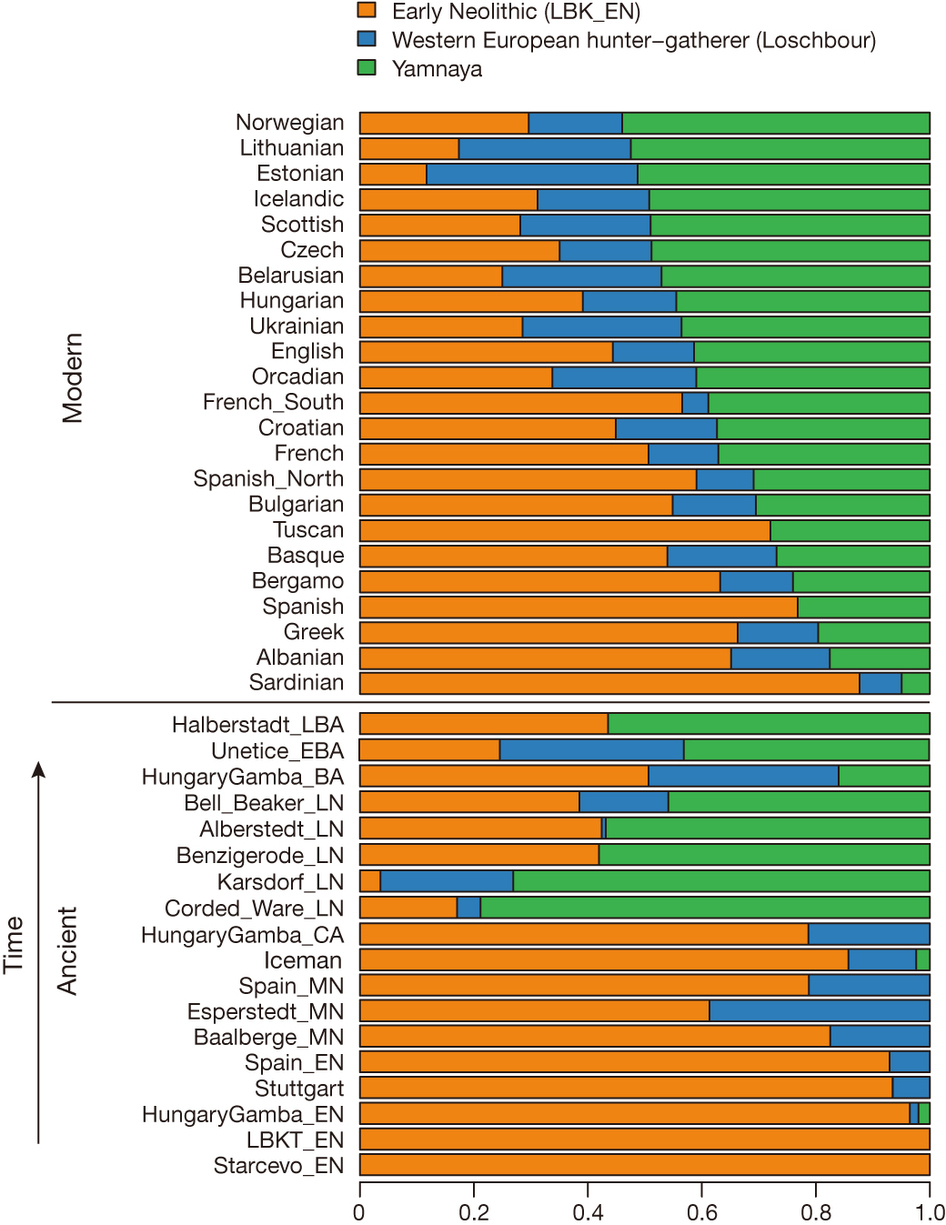
\includegraphics[width=5in, height=5in]{../nature14317-f3.png}
\caption{Haak et al (2015): modern and ancient European populations can be written as a mixture of Yamanaya, LBK-EN and Loschbour}
\end{figure}

To estimate the admixture proportions ($\alpha_i$), Haak et al. used the "F4 statistics" concept (a statistic pioneered from their group) where,

$$f_4(Test; A; B, C) \approx \sum_{i=1}^N \alpha_i f_4(Ref_i; A; B,C)$$

with $\sum_{i=1}^N \alpha_i = 1$ and $\alpha_i \geq 0$ and $Test$ represent the allele frequency of the test population (which are modern day populations in this case) and $A$,$B$,$C$ are the allele frequencies of the "outgroups"" populations. $Ref_i$ is the allele frequency of the $ith$ ancient population.

There are $n{n-1 \choose 2}$ combinations of $A,B,C$ Thus, for one test population, they have $n{n-1 \choose 2}$ linear equations and solve for $\alpha_i$ by least squares. 

Why do we feel that there's room for an alternate analysis? We cite the following reasons

\begin{itemize}

\item We wanted to apply a more standard approach that is easier to interpret. We know that the STRUCTURE model is one such approach and has been proved to be effective for population genetic data-sets. 

\item We would like to cluster the data using the genotype data so as to get a better feel of within group heterogeneity, instead of using  allele frequencies which is the case for the F4 approach. 

\item Haak et al fixed 3 source populations (Yamanya, LBK-EN, Loschbour) and expressed the modern day Europeans as a mixture of these 3 ancient source populations. From this analysis, Haak et al claim that Europeans therefore can be written as a mixture of just these 3 ancient populations. However, there might be a possibility that there are some unknown ancient populations which modern day populations derive significant ancestry from; something the authors did not investigate. 

\item There has been many other papers that apply ADMIXTURE to pooled ancient + modern day data that do not take account of the hierarchy of the pooled ancient + modern day data. 

\end{itemize}

\end{document}



